% Figure 1.5 (Session 1): classical antiferromagnetic order with and without frustration.
% The image is rendered by figures/blender/s1_5_neel_vs_spiral.py; the coordinates of the labels
% come from figures/blender/out/neel_vs_spiral_anchors.tex. Compile with:
%   pdflatex neel_vs_spiral.tex ; result moves to ../classical_magnetism/neel_vs_spiral.pdf
\documentclass[11pt,tikz,border=0pt]{standalone}
\usepackage{amsmath,amssymb,graphicx}
\usepackage{xcolor}
\definecolor{coursedark}{HTML}{1B2A4A}
\definecolor{costamber}{HTML}{B8620A}
\newlength{\figw}\setlength{\figw}{16.19cm}   % the text width of the notes (letter, 2.7 cm margins), so labels print at size

\begin{document}
\begin{tikzpicture}[lbl/.style={font=\small, text=coursedark}]
  \node[anchor=south west, inner sep=0pt] at (0,0)
    {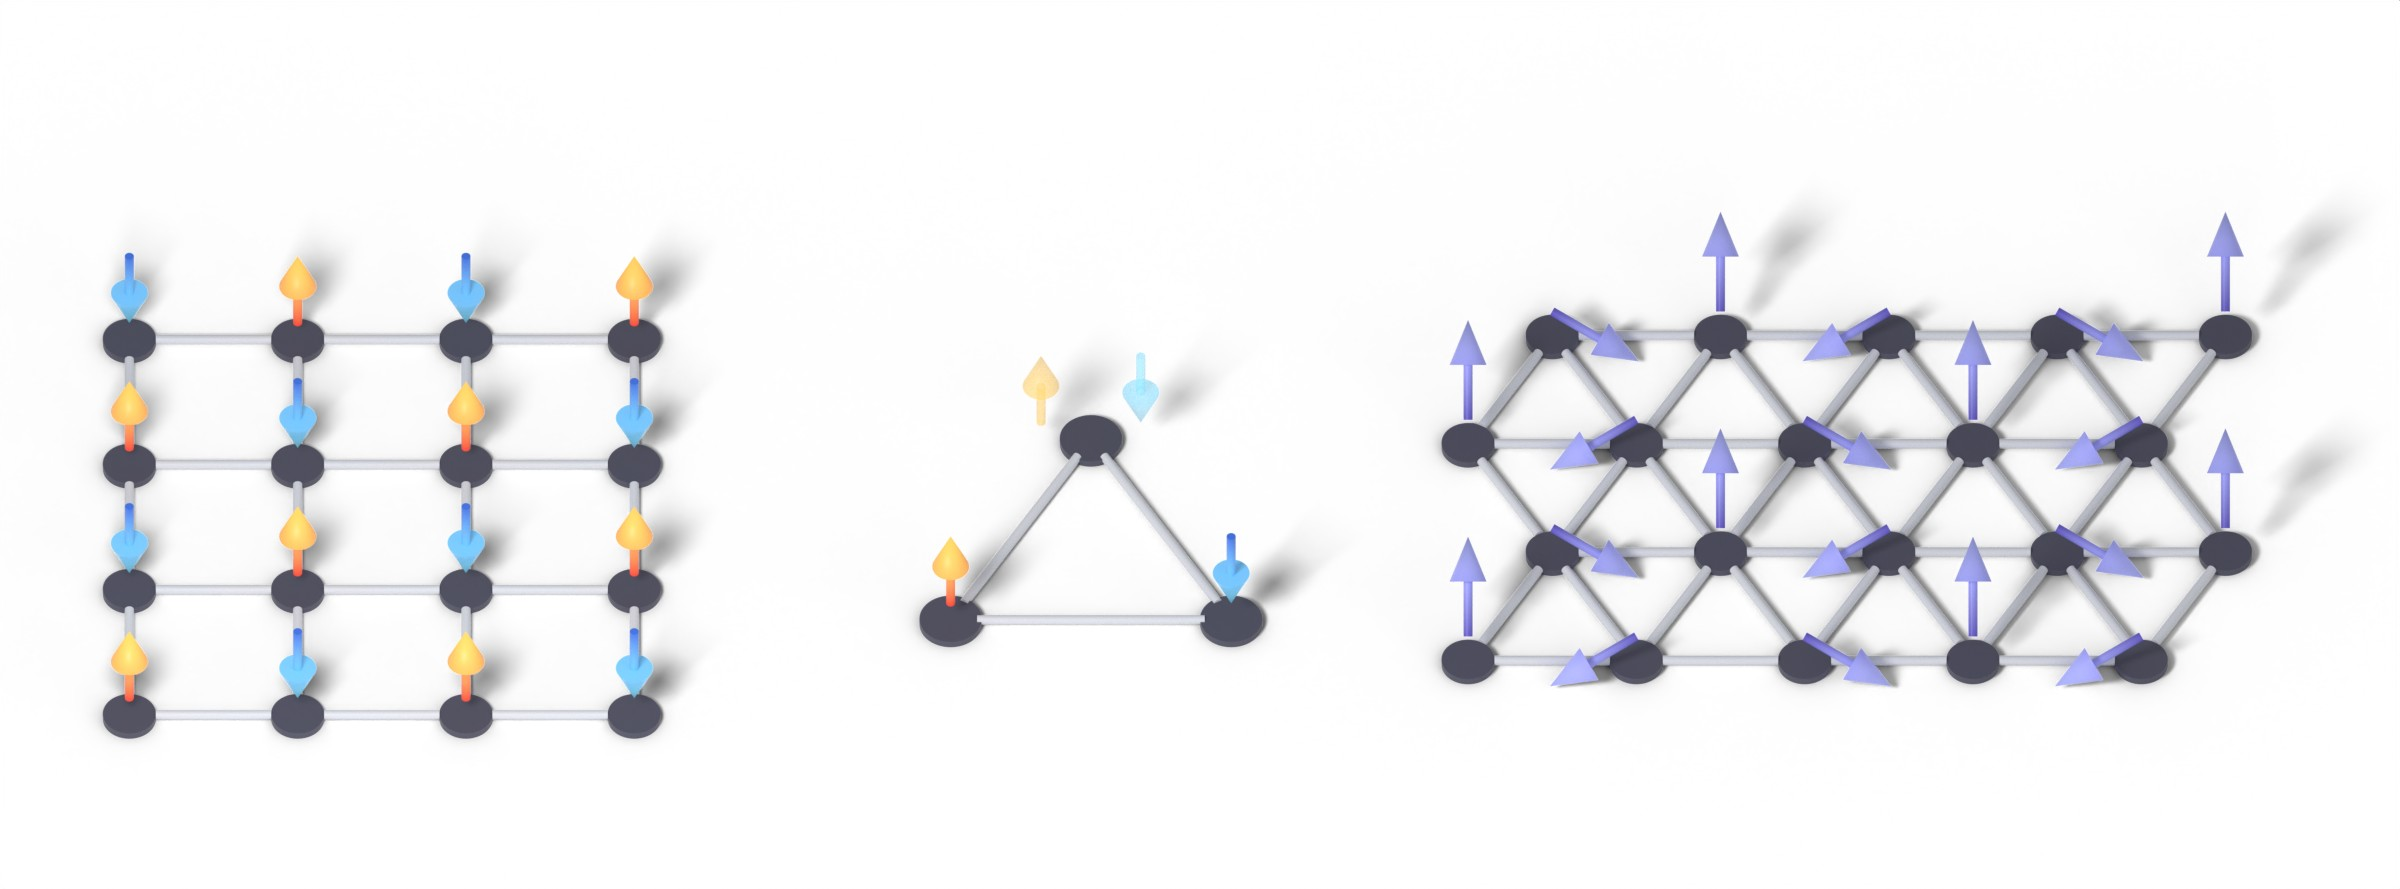
\includegraphics[width=\figw]{../blender/out/neel_vs_spiral.jpg}};
  %% written by figlib.py; x and y in units of the image width
\coordinate (a) at (0.0162\figw,0.3276\figw);
\coordinate (la) at (0.1591\figw,0.0515\figw);
\coordinate (q) at (0.4903\figw,0.2234\figw);
\coordinate (b) at (0.3701\figw,0.3276\figw);
\coordinate (lb) at (0.4545\figw,0.0911\figw);
\coordinate (c) at (0.6006\figw,0.3276\figw);
\coordinate (lc) at (0.7695\figw,0.0742\figw);

  \node[lbl, font=\normalsize, anchor=west] at (a) {(a)};
  \node[lbl, font=\normalsize, anchor=west] at (b) {(b)};
  \node[lbl, font=\normalsize, anchor=west] at (c) {(c)};
  \node[lbl, anchor=west, font=\normalsize] at (q) {?};
  \node[lbl, anchor=north] at (la) {square lattice, N\'eel};
  \node[lbl, anchor=north] at (lb) {one triangle};
  \node[lbl, anchor=north] at (lc) {triangular lattice, $120^\circ$};
\end{tikzpicture}
\end{document}
